\documentclass{standalone}

\usepackage{amssymb}
\usepackage{amsthm}
\usepackage{amsmath}


\usepackage{tikz}
\usetikzlibrary{shapes,backgrounds,calc,patterns}


\begin{document}
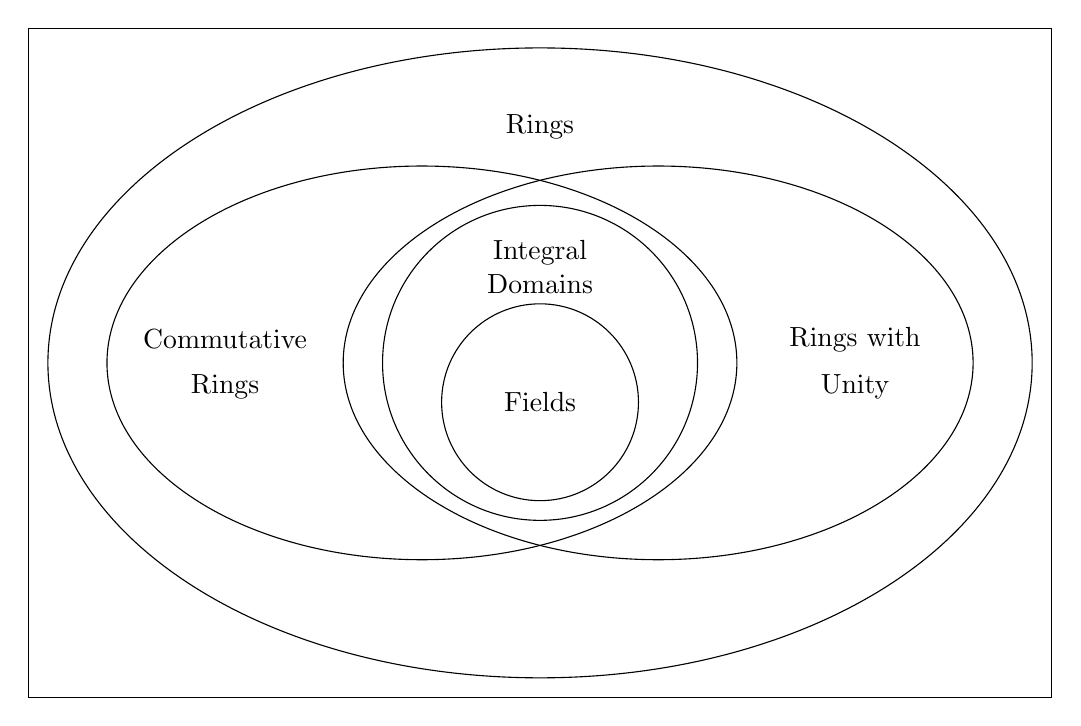
\begin{tikzpicture}
\draw (-6.5,4.25) rectangle (6.5,-4.25);
\draw (0,-.5) circle (1.25);
\draw (0,0) circle (2);
\draw (0,0) ellipse (6.25 and 4);
\draw (1.5,0) ellipse (4 and 2.5);
\draw (-1.5,0) ellipse (4 and 2.5);
\node at (0,3) {Rings};
\node at (0,-.5) {Fields};
\node at (0,1.4) {Integral};
\node at (0,1) {Domains};
\node at (4,.3) {Rings with};
\node at (4,-.3) {Unity};
\node at (-4,.3) {Commutative};
\node at (-4,-.3) {Rings};
\end{tikzpicture}
\end{document}